\documentclass[12pt,a4paper]{article}

% Idioma y codificación (si escribes en español)
\usepackage[utf8]{inputenc}
\usepackage[spanish]{babel}

% Matemáticas y Física
\usepackage{amsmath, amssymb, amsthm}
\usepackage{mathtools}
\usepackage{bm}
\usepackage{physics}
\usepackage{cancel}

% Gráficos y Tablas
\usepackage{graphicx}
\usepackage{booktabs}
\usepackage{float}
\usepackage[font=small, labelfont=bf]{caption}

% Referencias (hyperref siempre debe ser de los últimos)
\usepackage{hyperref}
\usepackage{cleveref}      % colors

\begin{document}

\section{Dinámica del sistema}

Este TFG se basa en el estudio y análisis de una red neuronal que evoluciona mediante una dinámica anti-hebbiana \eqref{dinamica X}, \eqref{dinamica W}. 

\begin{equation}
  \dot{X} = WX\\
  \label{dinamica X}
\end{equation}
    
\begin{equation}
  \dot{W} = \alpha (I - XX^T)
  \label{dinamica W}
\end{equation}

\subsection{Dinámica de \texorpdfstring{$W$}{W} y sus autovalores}

Como PATATA se observa de la dinámica de $W$ \eqref{dinamica W}, la única parte de la matriz que evoluciona es la parte simétrica, por lo que como los autovalores de una matriz simétrica son puramente reales  y de la antisimétrica puramente imaginarios, es razonable pensar que en los autovalores de la matriz  $W$ solo (o mayormente) evolucione la parte real mientras que la imaginaria quede perturbada mínimamente (ver Figura \ref{fig:evolucion autovalores}). Los resultados replican los de \cite{magnasco2009}. 

Además la frecuencia de las oscilaciones de la parte real de los autovalores muestra una dependencia lineal con $\sqrt{\alpha}$ como indica \cite{magnasco2009}

\begin{figure}[H]
  \centering
  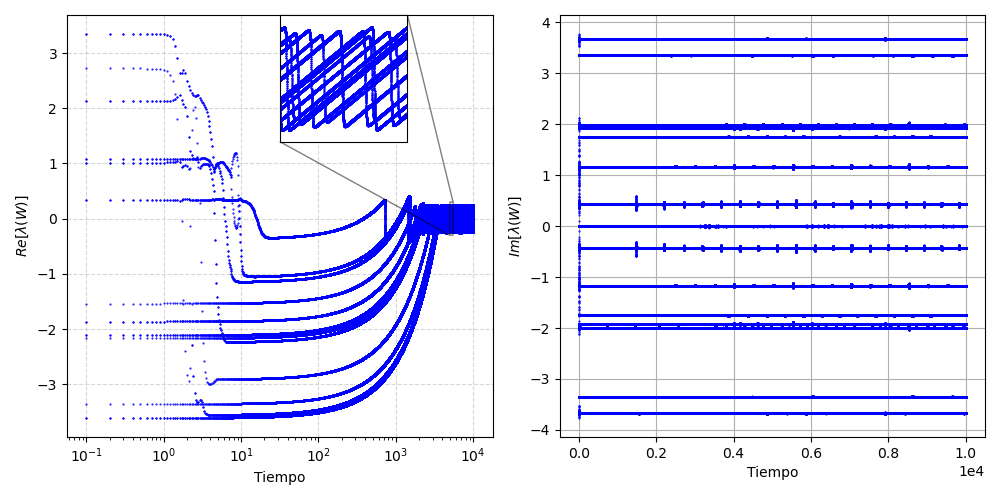
\includegraphics[width=.9\linewidth]{../Animaciones y figuras/Evolucion autovalores.png}
            
  \caption{Evolución temporal de la parte real (\textbf{Izda.}) e imaginaria (\textbf{Dcha.}) 
  de los autovalores de la matriz de conexiones, $W$, con entradas $W_{ij}\sim \mathcal{N}(0, 1)$, para $N=20$, $\alpha = 0.001$. La parte real de los autovalores positivos disminuye rápidamente en escala de tiempo $t_{+} \simeq 1$, mientras que la parte negativa aumenta hasta 0 en escalas de $t_{-} \simeq 10^3 = \frac{1}{\alpha}$, y como para tiempos mayores que $t_{-}$ la parte real oscila en torno a 0. La parte imaginaria se mantiene constante en promedio excepto por ligeras perturbaciones que ocurren cuando la parte real del autovalor alcanza el máximo.}

  \label{fig:evolucion autovalores}
\end{figure}

\section{Actividad neuronal}
\subsection{PCA}
Para comprobar si aparece criticidad, una vez el sistema se ha estabilizado en el régimen en el que los autovalores oscilan en torno al 0 se ha llevado a cabo un análisis componentes principales de la red neuronal calculando la distribución de autovalores del espectro de la matriz de covarianza de $X$ a lo largo del tiempo buscando una ley de potencias.

\begin{figure}[H]
  \centering
  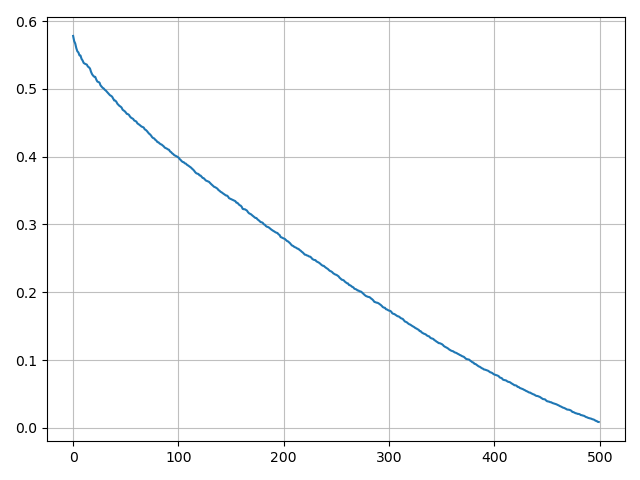
\includegraphics[width=0.8\linewidth]{../Simulaciones en Python/cov_eig.png}
  \caption{Autovalores de la matriz de covarianza de la serie temporal de $X$ ordenados de mayor a menor en escala lineal para $N=500$, $\alpha=0.0001$. No se ajusta a una ley de potencias, lo que indica la ausencia de criticidad del sistema.}
\end{figure}


\subsection{Análisis de los picos de actividad}
Analizando la serie temporal de $X$ y la de los autovalores de $W$ se observa una correlación entre los picos de actividad en $X$ y los puntos en los que los autovalores de $W$ ``caen'' desde $Re(\lambda) > 0$ hasta $Re(\lambda) < 0$. Intuitivamente cuando $X \sim 0$, $W$ y por tanto sus autovalores crecen de forma lineal con $\dot{W} = \alpha$, asimismo $X$ evoluciona de forma exponencial con la parte real de $\lambda$, por lo que una vez que $Re(\lambda) > 0$, $X$ crece exponencialmente hasta que $XX^T \gg I$, cuando aparece un pico en la actividad. Una vez que $X$ ha dejado de ser insignificante $W$ empieza a decrecer hasta hacerse $Re(\lambda) < 0$, por lo que genera que $X \sim 0$ y vuelve el ciclo. Este proceso se muestra en la Figura \ref{picos de actividad}

Como $X$ es una combinación lineal de los autovectores de $W$ este proceso se llevará a cabo con cada autovalor, por lo que para $N$ pequeño se verán picos diferenciados ya que la distancia entre caidas de autovalores es apreciable, mientras que para $N$ muy grandes, p.ej. 100, la distancia entre caidas de autovalores es tan pequeña que las excitaciones se solapan hasta asemejarse a ruido estocástico, pero conteniendo cierta periodicidad (la de las oscilaciones de los autovalores). 

\begin{figure}[H]
  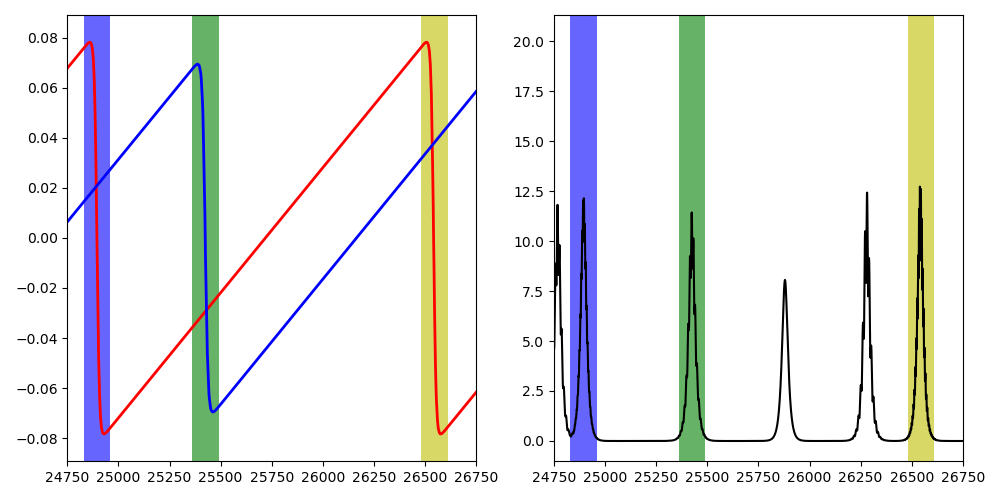
\includegraphics[width=\linewidth]{../Simulaciones en Python/Picos.png}
  \caption{Representación de la correlación entre caidas de autovalores y picos de actividad para $N=7$, $\alpha=0.0001$. \textbf{Izda.:} Evolución de dos de los autovalores de la matriz de conexiones, resaltando las caidas de $Re(\lambda)$ para cada uno de ellos. \textbf{Dcha.:} Actividad de la red calculada como $|X|^2$, donde se observa cómo los picos corresponden con las caidas en el espacio de autovalores. Los picos sin resaltar corresponden con otros autovalores que no se muestran en la gráfica.}
  \label{picos de actividad}
\end{figure}

\bibliographystyle{unsrt}
\bibliography{bibliografia}
\end{document}